%%%%%%%%%%%%%%%%%%%%%%%%%%%%%%%%%%%%%%%%%%%%%%%%%%%%%%%%%%%%%%%%%%%%%%%%
%% Customizações do abnTeX2 (http://abnTeX2.googlecode.com)           %%
%% para a Faculdade Cenecista de Osório - CNEC/FACOS                  %%
%%                                                                    %%
%% This work may be distributed and/or modified under the             %% 
%% conditions of the LaTeX Project Public License, either version 1.3 %%
%% of this license or (at your option) any later version.             %%
%% The latest version of this license is in                           %%
%%   http://www.latex-project.org/lppl.txt                            %%
%% and version 1.3 or later is part of all distributions of LaTeX     %%
%% version 2005/12/01 or later.                                       %%
%%                                                                    %%
%% This work has the LPPL maintenance status `maintained'.            %%
%%                                                                    %%
%% The Current Maintainer of this work is Augusto Weiand              %%
%%                                                                    %%
%% Project available on: https://github.com/aweiand/facostex          %%
%%                                                                    %%
%% Further information about abnTeX2                                  %%
%% are available on http://abntex2.googlecode.com/                    %%
%%                                                                    %%
%%%%%%%%%%%%%%%%%%%%%%%%%%%%%%%%%%%%%%%%%%%%%%%%%%%%%%%%%%%%%%%%%%%%%%%%

\documentclass[        
    a4paper,          % Tamanho da folha A4
    12pt,             % Tamanho da fonte 12pt
    chapter=TITLE,    % Todos os capitulos devem ter caixa alta
    section=TITLE,    % Todas as secoes devem ter caixa alta
    oneside,          % Usada para impressao em apenas uma face do papel
    english,          % Hifenizacoes em ingles
    spanish,          % Hifenizacoes em espanhol
    brazil            % Ultimo idioma eh o idioma padrao do documento
]{abntex2}

%%%%%%%%%%%%%%%%%%%%%%%%%%%%%%%%%%%%%%%%%%%%%%%%%%%%%%%%%%%%%%%%%%%%%%%%
%% Customizações do abnTeX2 (http://abnTeX2.googlecode.com)           %%
%% para a Faculdade Cenecista de Osório - CNEC/FACOS                  %%
%%                                                                    %%
%% This work may be distributed and/or modified under the             %% 
%% conditions of the LaTeX Project Public License, either version 1.3 %%
%% of this license or (at your option) any later version.             %%
%% The latest version of this license is in                           %%
%%   http://www.latex-project.org/lppl.txt                            %%
%% and version 1.3 or later is part of all distributions of LaTeX     %%
%% version 2005/12/01 or later.                                       %%
%%                                                                    %%
%% This work has the LPPL maintenance status `maintained'.            %%
%%                                                                    %%
%% The Current Maintainer of this work is Augusto Weiand              %%
%%                                                                    %%
%% Project available on: https://github.com/aweiand/facostex          %%
%%                                                                    %%
%% Further information about abnTeX2                                  %%
%% are available on http://abntex2.googlecode.com/                    %%
%%                                                                    %%
%%%%%%%%%%%%%%%%%%%%%%%%%%%%%%%%%%%%%%%%%%%%%%%%%%%%%%%%%%%%%%%%%%%%%%%%

% \documentclass[        
%     a4paper,          % Tamanho da folha A4
%     12pt,             % Tamanho da fonte 12pt
%     chapter=TITLE,    % Todos os capitulos devem ter caixa alta
%     section=TITLE,    % Todas as secoes devem ter caixa alta
%     oneside,          % Usada para impressao em apenas uma face do papel
%     english,          % Hifenizacoes em ingles
%     spanish,          % Hifenizacoes em espanhol
%     brazil            % Ultimo idioma eh o idioma padrao do documento
% ]{abntex2}

% Importações de pacotes
\usepackage[utf8]{inputenc}                         % Acentuação direta
\usepackage[T1]{fontenc}                            % Codificação da fonte em 8 bits
\usepackage{graphicx}                               % Inserir figuras
\usepackage{amsfonts, amssymb, amsmath}             % Fonte e símbolos matemáticos
\usepackage{booktabs}                               % Comandos para tabelas
\usepackage{verbatim}                               % Texto é interpretado como escrito no documento
\usepackage{multirow, array}                        % Múltiplas linhas e colunas em tabelas
\usepackage{indentfirst}                            % Endenta o primeiro parágrafo de cada seção.
\usepackage{listings}                               % Utilizar codigo fonte no documento
\usepackage{xcolor}
\usepackage{microtype}                              % Para melhorias de justificação?
\usepackage[portuguese,ruled,lined]{algorithm2e}    % Escrever algoritmos
\usepackage{algorithmic}                            % Criar Algoritmos  
%\usepackage{float}                                  % Utilizado para criação de floats
\usepackage{amsgen}
\usepackage{lipsum}                                 % Usar a simulação de texto Lorem Ipsum
%\usepackage{titlesec}                               % Permite alterar os títulos do documento
\usepackage{tocloft}                                % Permite alterar a formatação do Sumário
\usepackage{etoolbox}                               % Usado para alterar a fonte da Section no Sumário
\usepackage[nogroupskip,nonumberlist,acronym]{glossaries}                % Permite fazer o glossario
\usepackage{caption}                                % Altera o comportamento da tag caption
\usepackage[alf, abnt-emphasize=bf, bibjustif, recuo=0cm, abnt-etal-cite=2, abnt-etal-list=0]{abntex2cite}  % Citações padrão ABNT
%\usepackage[bottom]{footmisc}                      % Mantém as notas de rodapé sempre na mesma posição
%\usepackage{times}                                 % Usa a fonte Times
\usepackage{mathptmx}                               % Usa a fonte Times New Roman										
%\usepackage{lmodern}                               % Usa a fonte Latin Modern
%\usepackage{subfig}                                % Posicionamento de figuras
%\usepackage{scalefnt}                              % Permite redimensionar tamanho da fonte
%\usepackage{color, colortbl}                       % Comandos de cores
%\usepackage{lscape}                                % Permite páginas em modo "paisagem"
%\usepackage{ae, aecompl}                           % Fontes de alta qualidade
%\usepackage{picinpar}                              % Dispor imagens em parágrafos
%\usepackage{latexsym}                              % Símbolos matemáticos
%\usepackage{upgreek}                               % Fonte letras gregas
\usepackage{appendix}                               % Gerar o apendice no final do documento
\usepackage{paracol}                                % Criar paragrafos sem identacao
\usepackage{lib/facostex}		                    % Biblioteca com as normas da UECE para trabalhos academicos
\usepackage{pdfpages}                               % Incluir pdf no documento
\usepackage{amsmath}                                % Usar equacoes matematicas

% Organiza e gera a lista de abreviaturas, simbolos e glossario
\makeglossaries

% Gera o Indice do documento
\makeindex


%%%%%%%%%%%%%%%%%%%%%%%%%%%%%%%%%%%%%%%%%%%%%%%%%%%%%
%%          Configuracoes do facosTex              %%
%%%%%%%%%%%%%%%%%%%%%%%%%%%%%%%%%%%%%%%%%%%%%%%%%%%%%

% Opcoes disponiveis

\trabalhoacademico{tccgraduacao}
%\trabalhoacademico{tccespecializacao}

% Define se o trabalho eh uma qualificacao
% Coloque 'nao' para versao final do trabalho

\ehqualificacao{nao}

% Remove as bordas vermelhas e verdes do PDF gerado
% Coloque 'sim' pare remover

\removerbordasdohyperlink{sim} 

% Adiciona a cor Azul a todos os hyperlinks

\cordohyperlink{nao}

%%%%%%%%%%%%%%%%%%%%%%%%%%%%%%%%%%%%%%%%%%%%%%%%%%%%%
%%          Informação sobre a IES                 %%
%%%%%%%%%%%%%%%%%%%%%%%%%%%%%%%%%%%%%%%%%%%%%%%%%%%%%

\ies{Faculdade Cenecista de Osório}
\iessigla{FACOS}
\centro{Campanha Nacional das Escolas da Comunidade}

%%%%%%%%%%%%%%%%%%%%%%%%%%%%%%%%%%%%%%%%%%%%%%%%%%%%%
%%        Informação para TCC de Graduacao         %%
%%%%%%%%%%%%%%%%%%%%%%%%%%%%%%%%%%%%%%%%%%%%%%%%%%%%%

\graduacaoem{Licenciatura em Informática}
\habilitacao{licenciado} % Pode colocar tambem 'bacharel'

%%%%%%%%%%%%%%%%%%%%%%%%%%%%%%%%%%%%%%%%%%%%%%%%%%%%%
%%     Informação para TCC de Especializacao       %%
%%%%%%%%%%%%%%%%%%%%%%%%%%%%%%%%%%%%%%%%%%%%%%%%%%%%%

% \especializacaoem{Alfabetização de Crianças}


%%%%%%%%%%%%%%%%%%%%%%%%%%%%%%%%%%%%%%%%%%%%%%
%%  Informação relacionadas ao trabalho     %%
%%%%%%%%%%%%%%%%%%%%%%%%%%%%%%%%%%%%%%%%%%%%%%

\autor{Nome Sobrenome}
\titulo{Título do Trabalho}
\data{2015}
\local{Osório}

% Exemplo: \dataaprovacao{01 de Janeiro de 2012}
\dataaprovacao{}

%%%%%%%%%%%%%%%%%%%%%%%%%%%%%%%%%%%%%%%%%%%%%
%%     Informação sobre o Orientador       %%
%%%%%%%%%%%%%%%%%%%%%%%%%%%%%%%%%%%%%%%%%%%%%

\orientador{Nome do seu Orientador}
\orientadories{Faculdade Cenecista de Osório}
% \orientadorcentro{Campanha Nacional das Escolas da Comunidade}
\orientadorfeminino{nao} % Coloque 'sim' se for do sexo feminino

%%%%%%%%%%%%%%%%%%%%%%%%%%%%%%%%%%%%%%%%%%%%%
%%      Informação sobre o Co-orientador   %%
%%%%%%%%%%%%%%%%%%%%%%%%%%%%%%%%%%%%%%%%%%%%%

% Deixe o nome do coorientador em branco para remover do documento

\coorientador{}
\coorientadories{Universidade Co-orientador - SIGLA}
\coorientadorcentro{Centro do Co-orientador - SIGLA}
\coorientadorfeminino{nao} % Coloque 'sim' se for do sexo feminino

%%%%%%%%%%%%%%%%%%%%%%%%%%%%%%%%%%%%%%%%%%%%%
%%      Informação sobre a banca           %%
%%%%%%%%%%%%%%%%%%%%%%%%%%%%%%%%%%%%%%%%%%%%%

% Atenção! Deixe o nome do membro da banca para remover da folha de aprovacao

% Exemplo de uso:
% \membrodabancadois{Prof. Dr. Fulano de Tal}
% \membrodabancadoisies{Universidade Estadual do Ceará - UECE}

\membrodabancadois{Membro da Banca Dois}
\membrodabancadoiscentro{Faculdade de Filosofia Dom Aureliano Matos – FAFIDAM}
\membrodabancadoisies{Universidade do Membro da Banca Dois - SIGLA}
\membrodabancatres{Membro da Banca Três}
\membrodabancatrescentro{Centro de Ciências e Tecnologia - CCT}
\membrodabancatresies{Universidade do Membro da Banca Três - SIGLA}
\membrodabancaquatro{Membro da Banca Quatro}
\membrodabancaquatrocentro{Centro de Ciências e Tecnologia - CCT}
\membrodabancaquatroies{Universidade do Membro da Banca Quatro - SIGLA}


\begin{document}	

	% Elementos pré-textuais
	\imprimircapa
	\imprimirfolhaderosto{}
    % \imprimirfichacatalografica{elementos-pre-textuais/ficha-catalografica}	
% 	\imprimirerrata{elementos-pre-textuais/errata}
    \imprimirfolhadeaprovacao
	\imprimirdedicatoria{elementos-pre-textuais/dedicatoria}
	\imprimiragradecimentos{elementos-pre-textuais/agradecimentos}
	\imprimirepigrafe{elementos-pre-textuais/epigrafe}
	\imprimirresumo{elementos-pre-textuais/resumo}
	\imprimirabstract{elementos-pre-textuais/abstract}
	\imprimirlistadeilustracoes
% 	\imprimirlistadetabelas
% 	\imprimirlistadequadros
% 	\imprimirlistadealgoritmos
% 	\imprimirlistadecodigosfonte
% 	\imprimirlistadeabreviaturasesiglas	
% 	\imprimirlistadesimbolos{elementos-pre-textuais/lista-de-simbolos}   
	\imprimirsumario
	
	%Elementos textuais
	\textual
	\chapter{Introdução}
\label{cap:introducao}

Integer non lacinia magna. Aenean tempor lorem tellus, non sodales nisl commodo ut. Proin mattis placerat risus sit amet laoreet. Praesent sapien arcu, maximus ac fringilla efficitur, vulputate faucibus sem. Donec aliquet velit eros, sit amet elementum dolor pharetra eget. Integer eget mattis libero.


\section{Motivação}
\label{sec:motivacao}

Integer non lacinia magna. Aenean tempor lorem tellus, non sodales nisl commodo ut. Proin mattis placerat risus sit amet laoreet. Praesent sapien arcu, maximus ac fringilla efficitur, vulputate faucibus sem. Donec aliquet velit eros, sit amet elementum dolor pharetra eget. Integer eget mattis libero.

Integer non lacinia magna. Aenean tempor lorem tellus, non sodales nisl commodo ut. Proin mattis placerat risus sit amet laoreet. Praesent sapien arcu, maximus ac fringilla efficitur, vulputate faucibus sem. Donec aliquet velit eros, sit amet elementum dolor pharetra eget. Integer eget mattis libero.

Integer non lacinia magna. Aenean tempor lorem tellus, non sodales nisl commodo ut. Proin mattis placerat risus sit amet laoreet. Praesent sapien arcu, maximus ac fringilla efficitur, vulputate faucibus sem. Donec aliquet velit eros, sit amet elementum dolor pharetra eget. Integer eget mattis libero.

\section{Objetivos}
\label{sec:objetivos}

Interdum et malesuada fames ac ante ipsum primis in faucibus. Lorem ipsum dolor sit amet, consectetur adipiscing elit. Ut ex tellus, sodales in euismod at, ultricies quis leo.

\subsection{Objetivo Geral}
\label{sec:objetivo-geral}

Integer imperdiet ac magna eu pulvinar. Aliquam erat volutpat. Etiam molestie, nulla a egestas aliquet, velit augue congue metus, et ultricies metus massa vel nibh. Vivamus viverra commodo finibus. Nam elementum convallis accumsan. Quisque tincidunt purus nisl, tincidunt ultricies odio ultrices eu.

\subsection{Objetivos Específicos}
\label{sec:objetivos-especificos}

Lorem ipsum dolor sit amet, consectetur adipiscing elit. Duis scelerisque, velit at facilisis hendrerit, dui eros lacinia metus, non maximus mi tortor ut lectus. Donec hendrerit leo ut consectetur tincidunt. 
	\chapter{Fundamentação Teórica}
\label{cap:fundamentacao-teorica}

Integer non lacinia magna. Aenean tempor lorem tellus, non sodales nisl commodo ut. Proin mattis placerat risus sit amet laoreet. Praesent sapien arcu, maximus ac fringilla efficitur, vulputate faucibus sem. Donec aliquet velit eros, sit amet elementum dolor pharetra eget. Integer eget mattis libero

\section{Fundamentação Teórica A}
\label{sec:fundamentacao-teorica-a}

Integer non lacinia magna. Aenean tempor lorem tellus, non sodales nisl commodo ut. Proin mattis placerat risus sit amet laoreet. Praesent sapien arcu, maximus ac fringilla efficitur, vulputate faucibus sem. Donec aliquet velit eros, sit amet elementum dolor pharetra eget. Integer eget mattis libero.

\begin{figure}[htb]
    \centering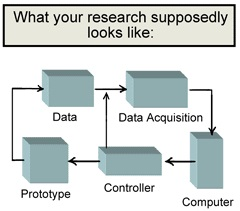
\includegraphics[width=.80\textwidth]{figuras/figura-1.jpg}
    \caption{\label{fig:exemplo-18}Exemplo.}
    
    Fonte: Exemplo%
\end{figure}
	
Integer non lacinia magna. Aenean tempor lorem tellus, non sodales nisl commodo ut. Proin mattis placerat risus sit amet laoreet. Praesent sapien arcu, maximus ac fringilla efficitur, vulputate faucibus sem. Donec aliquet velit eros, sit amet elementum dolor pharetra eget. Integer eget mattis libero.

Integer non lacinia magna. Aenean tempor lorem tellus, non sodales nisl commodo ut. Proin mattis placerat risus sit amet laoreet. Praesent sapien arcu, maximus ac fringilla efficitur, vulputate faucibus sem. Donec aliquet velit eros, sit amet elementum dolor pharetra eget. Integer eget mattis libero.


\section{Fundamentação Teórica B}
\label{sec:fundamentacao-teorica-b}

Integer non lacinia magna. Aenean tempor lorem tellus, non sodales nisl commodo ut. Proin mattis placerat risus sit amet laoreet. Praesent sapien arcu, maximus ac fringilla efficitur, vulputate faucibus sem. Donec aliquet velit eros, sit amet elementum dolor pharetra eget. Integer eget mattis libero. Praesent ex velit, pulvinar at massa vel, fermentum dictum mauris. Ut feugiat accumsan augue, et ultrices ipsum euismod vitae

\begin{figure}[htb]
    \centering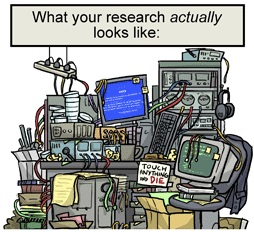
\includegraphics[width=.80\textwidth]{figuras/figura-2.jpg}
    \caption{\label{fig:exemplo-2}Exemplo.}
    
    Fonte: Exemplo%
\end{figure}

Nunc ac pretium dui. Mauris aliquam dapibus nulla ac mattis. Aenean non tortor volutpat, varius lectus vitae, accumsan nibh. Cras pretium vestibulum enim, id ullamcorper tortor ultrices non. Integer sodales viverra faucibus. Curabitur at dui lacinia, rhoncus lacus at, blandit metus. Integer scelerisque non enim quis ornare.

Duis faucibus, enim quis tincidunt pellentesque, nisl leo varius nulla, vitae tempus dui mauris ac ante. Quisque purus lorem, pharetra sit amet lobortis eu, vehicula vitae purus. Ut varius, erat nec vehicula elementum, risus est tempus justo, nec vulputate augue leo egestas metus.

\begin{figure}[htb]
    \centering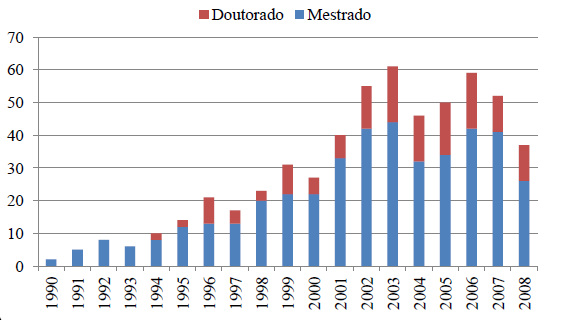
\includegraphics[width=.80\textwidth]{figuras/figura-3.png}
    \caption{\label{fig:exemplo-3}Exemplo.}
    
    Fonte: Exemplo%
\end{figure}

Integer non lacinia magna. Aenean tempor lorem tellus, non sodales nisl commodo ut. Proin mattis placerat risus sit amet laoreet. Praesent sapien arcu, maximus ac fringilla efficitur, vulputate faucibus sem. Donec aliquet velit eros, sit amet elementum dolor pharetra eget. Integer eget mattis libero.

\begin{table}[htb]
\centering
\caption{\label{tab:exemplo-tabela}Lista de trabalhos considerando as visualizações disponibilizadas}%
\resizebox{\textwidth}{!}{%
\begin{tabular}{|l|c|c|c|c|c|}
\hline
& \textbf{Sem Gráficos} & \textbf{Interatividade} & \textbf{Linha} & \textbf{Barra} & \textbf{Mapa de Calor} \\ \hline
Amershi e Conati                  &              & X              & X     &       & x     \\ \hline
Baruque et al.                    & X            &                &       &       &       \\ \hline
Bovo et al.                       & X            &                &       &       &       \\ \hline
Bravo e Ortigosa                  & X            &                &       &       &       \\ \hline
Chirioiu et al.                   &              & X              &       &       & X     \\ \hline
\end{tabular}
}
\end{table}
	
Duis faucibus, enim quis tincidunt pellentesque, nisl leo varius nulla, vitae tempus dui mauris ac ante. Quisque purus lorem, pharetra sit amet lobortis eu, vehicula vitae purus.
	\chapter{Trabalhos Relacionados}
\label{cap:trabalhos-relacionados}

Integer non lacinia magna. Aenean tempor lorem tellus, non sodales nisl commodo ut. Proin mattis placerat risus sit amet laoreet. Praesent sapien arcu, maximus ac fringilla efficitur, vulputate faucibus sem. Donec aliquet velit eros, sit amet elementum dolor pharetra eget. Integer eget mattis libero.

\section{Trabalho Relacionado A}
\label{sec:trabalho-relacionado-a}

Integer non lacinia magna. Aenean tempor lorem tellus, non sodales nisl commodo ut. Proin mattis placerat risus sit amet laoreet. Praesent sapien arcu, maximus ac fringilla efficitur, vulputate faucibus sem. Donec aliquet velit eros, sit amet elementum dolor pharetra eget. Integer eget mattis libero.

\begin{figure}[htb]
    \centering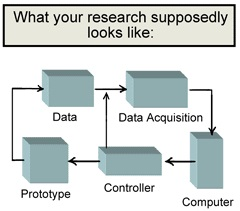
\includegraphics[width=.80\textwidth]{figuras/figura-1.jpg}
    \caption{\label{fig:exemplo-6}Exemplo.}
    
    Fonte: Exemplo%
\end{figure}
	
Integer non lacinia magna. Aenean tempor lorem tellus, non sodales nisl commodo ut. Proin mattis placerat risus sit amet laoreet. Praesent sapien arcu, maximus ac fringilla efficitur, vulputate faucibus sem. Donec aliquet velit eros, sit amet elementum dolor pharetra eget. Integer eget mattis libero.

\section{Trabalho Relacionado B}
\label{sec:trabalho-relacionado-b}

Integer non lacinia magna. Aenean tempor lorem tellus, non sodales nisl commodo ut. Proin mattis placerat risus sit amet laoreet. Praesent sapien arcu, maximus ac fringilla efficitur, vulputate faucibus sem. Donec aliquet velit eros, sit amet elementum dolor pharetra eget. Integer eget mattis libero. Praesent ex velit, pulvinar at massa vel, fermentum dictum mauris. Ut feugiat accumsan augue, et ultrices ipsum euismod vitae

\begin{figure}[htb]
    \centering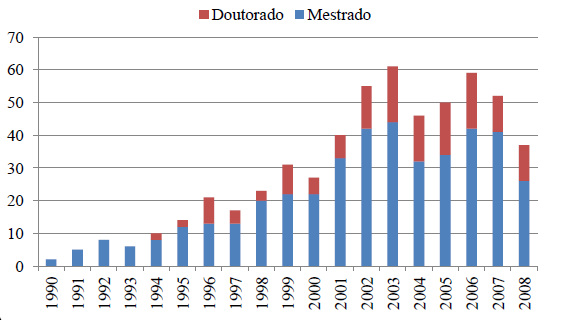
\includegraphics[width=.80\textwidth]{figuras/figura-3.png}
    \caption{\label{fig:exemplo-5}Exemplo.}
    
    Fonte: Exemplo%
\end{figure}

Nunc ac pretium dui. Mauris aliquam dapibus nulla ac mattis. Aenean non tortor volutpat, varius lectus vitae, accumsan nibh. Cras pretium vestibulum enim, id ullamcorper tortor ultrices non. Integer sodales viverra faucibus. Curabitur at dui lacinia, rhoncus lacus at, blandit metus. Integer scelerisque non enim quis ornare.


	\chapter{Metodologia}
\label{chap:metodologia}

Integer non lacinia magna. Aenean tempor lorem tellus, non sodales nisl commodo ut. Proin mattis placerat risus sit amet laoreet. Praesent sapien arcu, maximus ac fringilla efficitur, vulputate faucibus sem. Donec aliquet velit eros, sit amet elementum dolor pharetra eget. Integer eget mattis libero.

O autor \cite{lamport1986latex} e \cite{Maia2011} Integer non lacinia magna. Aenean tempor lorem tellus, non sodales nisl commodo ut. Proin mattis placerat risus sit amet laoreet. Praesent sapien arcu, maximus ac fringilla efficitur, vulputate faucibus sem. Donec aliquet velit eros, sit amet elementum dolor pharetra eget. Integer eget mattis libero.

Integer non lacinia magna. Aenean tempor lorem tellus, non sodales nisl commodo ut. Proin mattis placerat risus sit amet laoreet. Praesent sapien arcu, maximus ac fringilla efficitur, vulputate faucibus sem. Donec aliquet velit eros, sit amet elementum dolor pharetra eget. Integer eget mattis libero. \cite{Huetal2000}



\section{Usando Questões}


Lorem ipsum dolor sit amet, consectetur adipiscing elit. Nunc dictum sed tortor nec viverra. consectetur adipiscing elit. Nunc dictum sed tortor nec viverra.

\begin{questao}
	\item Esta é a primeira questão com alguns itens:
		\begin{enumerate}
			\item Este é o primeiro item
			\item Segundo item
		\end{enumerate}
	\item Esta é a segunda questão:
		\begin{enumerate}
			\item Este é o primeiro item
			\item Segundo item
		\end{enumerate}
	\item Lorem ipsum dolor sit amet, consectetur adipiscing elit. Nunc dictum sed tortor nec viverra. consectetur adipiscing elit. Nunc dictum sed tortor nec viverra.
		\begin{enumerate}
			\item consectetur
			\item adipiscing
			\item Nunc
			\item dictum
		\end{enumerate}
\end{questao}

	\chapter{Resultados}
\label{chap:resultados}

Integer non lacinia magna. Aenean tempor lorem tellus, non sodales nisl commodo ut. Proin mattis placerat risus sit amet laoreet. Praesent sapien arcu, maximus ac fringilla efficitur, vulputate faucibus sem. Donec aliquet velit eros, sit amet elementum dolor pharetra eget. Integer eget mattis libero.

\section{Resultados do Experimento A}
\label{sec:resultados-do-experimento-a}

Integer non lacinia magna. Aenean tempor lorem tellus, non sodales nisl commodo ut. Proin mattis placerat risus sit amet laoreet. Praesent sapien arcu, maximus ac fringilla efficitur, vulputate faucibus sem. Donec aliquet velit eros, sit amet elementum dolor pharetra eget. Integer eget mattis libero.

Integer non lacinia magna. Aenean tempor lorem tellus, non sodales nisl commodo ut. Proin mattis placerat risus sit amet laoreet. Praesent sapien arcu, maximus ac fringilla efficitur, vulputate faucibus sem. Donec aliquet velit eros, sit amet elementum dolor pharetra eget. Integer eget mattis libero.

Integer non lacinia magna. Aenean tempor lorem tellus, non sodales nisl commodo ut. Proin mattis placerat risus sit amet laoreet. Praesent sapien arcu, maximus ac fringilla efficitur, vulputate faucibus sem. Donec aliquet velit eros, sit amet elementum dolor pharetra eget. Integer eget mattis libero.

\section{Resultados do Experimento B}
\label{sec:resultados-do-experimento-b}

Integer non lacinia magna. Aenean tempor lorem tellus, non sodales nisl commodo ut. Proin mattis placerat risus sit amet laoreet. Praesent sapien arcu, maximus ac fringilla efficitur, vulputate faucibus sem. Donec aliquet velit eros, sit amet elementum dolor pharetra eget. Integer eget mattis libero.

\begin{table}[htb]
    \centering
    \caption{\label{tab:tabela-exemplo2}Tabela Exemplo 2}
    \begin{tabular}{lc}
        \textbf{Coluna 1} & \textbf{Coluna 2} \\
        Linha 1 Coluna 1  & Linha 1 Coluna 1  \\
        Linha 2 Coluna 1  & Linha 2 Coluna 2 
    \end{tabular}
\end{table}

Integer non lacinia magna. Aenean tempor lorem tellus, non sodales nisl commodo ut. Proin mattis placerat risus sit amet laoreet. Praesent sapien arcu, maximus ac fringilla efficitur, vulputate faucibus sem. Donec aliquet velit eros, sit amet elementum dolor pharetra eget. Integer eget mattis libero.
	\chapter{Conclusões e Trabalhos Futuros}
\label{chap:conclusoes-e-trabalhos-futuros}

Integer non lacinia magna. Aenean tempor lorem tellus, non sodales nisl commodo ut. Proin mattis placerat risus sit amet laoreet. Praesent sapien arcu, maximus ac fringilla efficitur, vulputate faucibus sem. Donec aliquet velit eros, sit amet elementum dolor pharetra eget. Integer eget mattis libero.

Integer non lacinia magna. Aenean tempor lorem tellus, non sodales nisl commodo ut. Proin mattis placerat risus sit amet laoreet. Praesent sapien arcu, maximus ac fringilla efficitur, vulputate faucibus sem. Donec aliquet velit eros, sit amet elementum dolor pharetra eget. Integer eget mattis libero.

Integer non lacinia magna. Aenean tempor lorem tellus, non sodales nisl commodo ut. Proin mattis placerat risus sit amet laoreet. Praesent sapien arcu, maximus ac fringilla efficitur, vulputate faucibus sem. Donec aliquet velit eros, sit amet elementum dolor pharetra eget. Integer eget mattis libero.


\section{Contribuições do Trabalho}
\label{sec:contribuicoes-do-trabalho}

Integer non lacinia magna. Aenean tempor lorem tellus, non sodales nisl commodo ut. Proin mattis placerat risus sit amet laoreet. Praesent sapien arcu, maximus ac fringilla efficitur, vulputate faucibus sem. Donec aliquet velit eros, sit amet elementum dolor pharetra eget. Integer eget mattis libero.


\section{Limitações}
\label{sec:limitacoes}

Integer non lacinia magna. Aenean tempor lorem tellus, non sodales nisl commodo ut. Proin mattis placerat risus sit amet laoreet. Praesent sapien arcu, maximus ac fringilla efficitur, vulputate faucibus sem. Donec aliquet velit eros, sit amet elementum dolor pharetra eget. Integer eget mattis libero.

Integer non lacinia magna. Aenean tempor lorem tellus, non sodales nisl commodo ut. Proin mattis placerat risus sit amet laoreet. Praesent sapien arcu, maximus ac fringilla efficitur, vulputate faucibus sem. Donec aliquet velit eros, sit amet elementum dolor pharetra eget. Integer eget mattis libero.


\section{Trabalhos Futuros}
\label{sec:trabalhos-futuros}

Integer non lacinia magna. Aenean tempor lorem tellus, non sodales nisl commodo ut. Proin mattis placerat risus sit amet laoreet. Praesent sapien arcu, maximus ac fringilla efficitur, vulputate faucibus sem. Donec aliquet velit eros, sit amet elementum dolor pharetra eget. Integer eget mattis libero.




	
	%Elementos pós-textuais	
	\bibliography{elementos-pos-textuais/referencias}
	\imprimirglossario	
	\imprimirapendices
		% Adicione aqui os apendices do seu trabalho
		\apendice{Lorem Ipsum}
\label{ap:lorem-ipsum}

\lipsum[1]
	\imprimiranexos
		% Adicione aqui os anexos do seu trabalho
		\anexo{Exemplo de Anexo}
\label{an:exemplo-de-anexo}

\lipsum[13]
	\imprimirindice

\end{document}